
%\setbeamertemplate{background canvas}{%
%    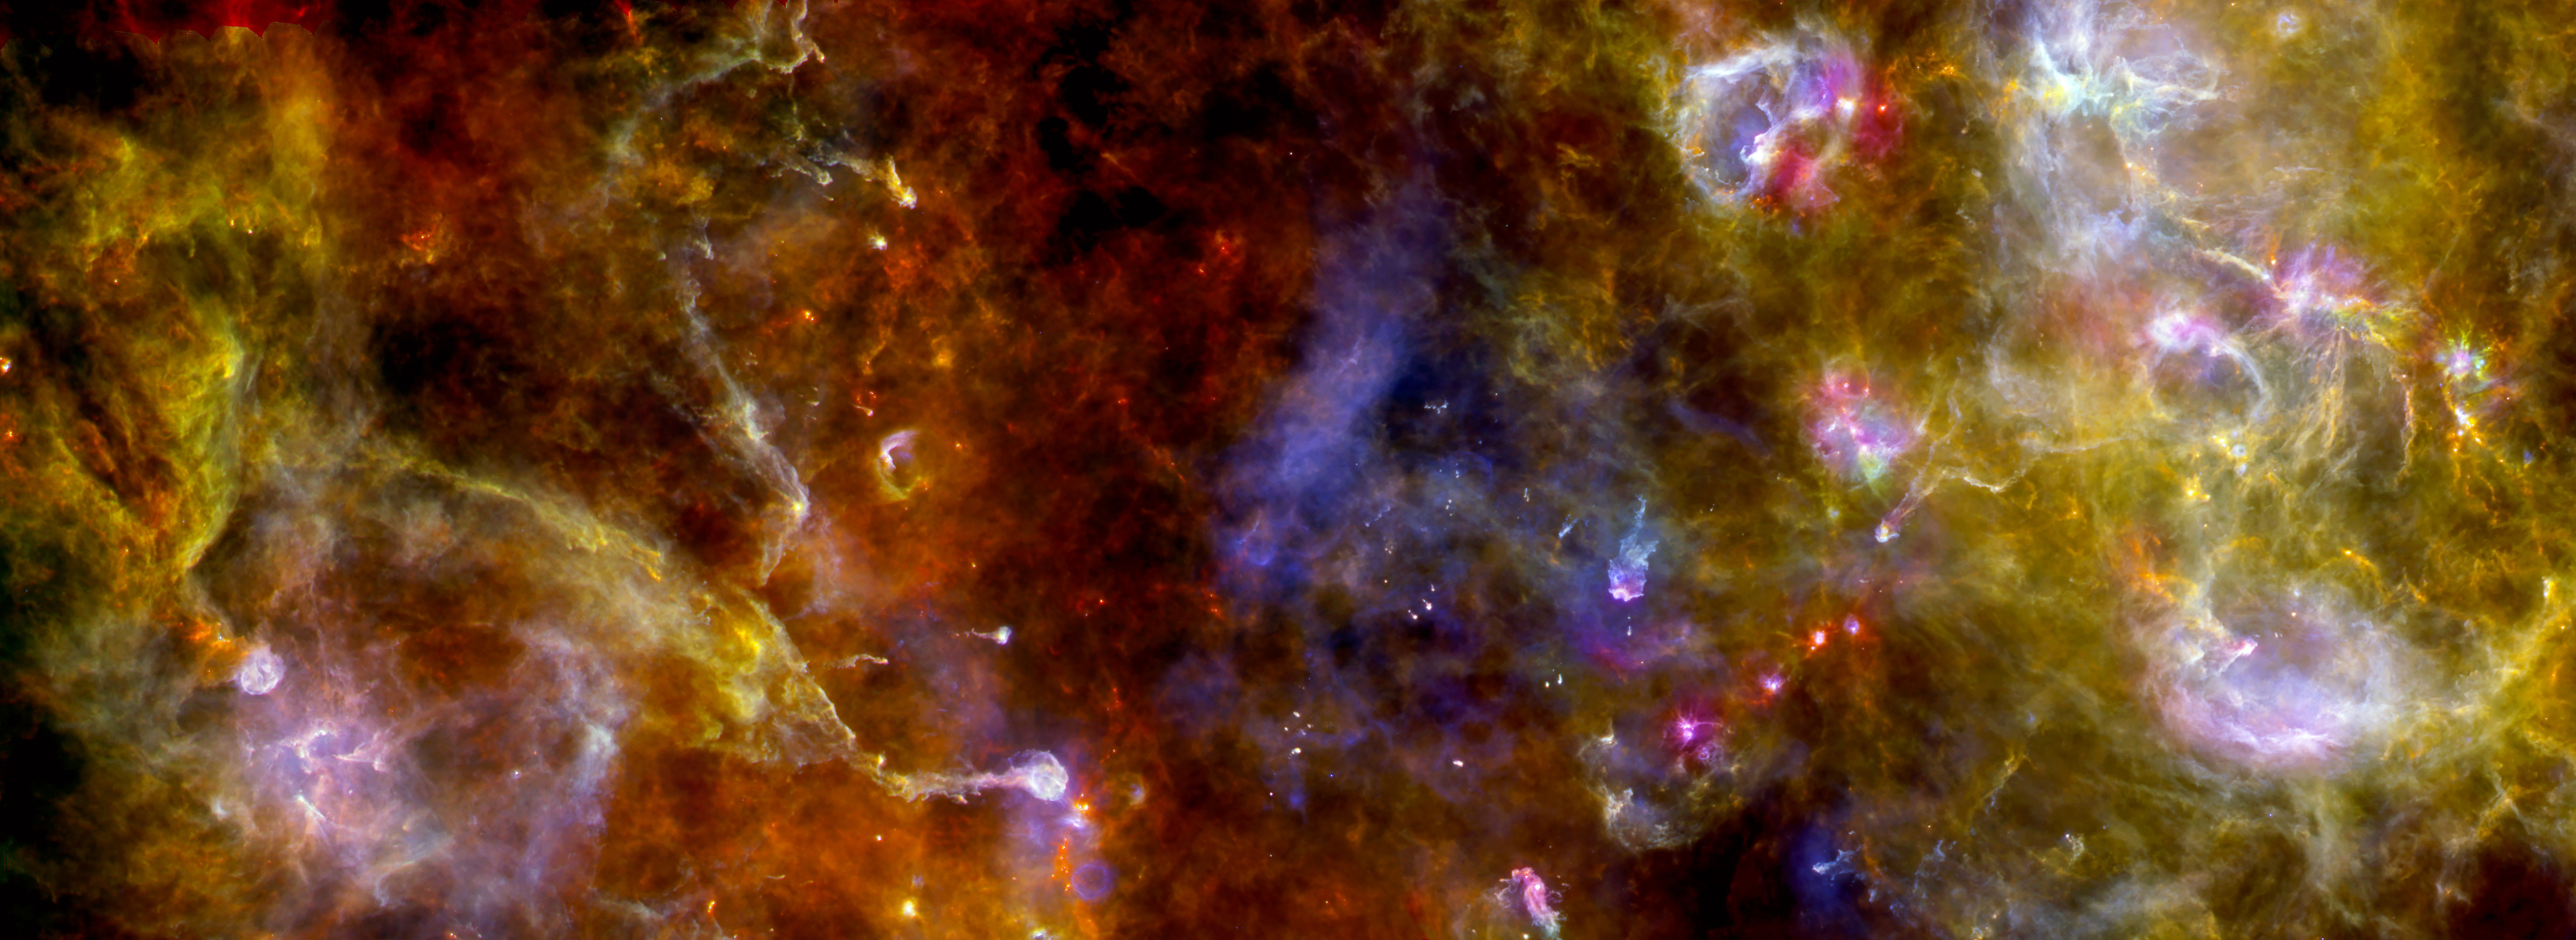
\includegraphics[width=\paperwidth,height=\paperheight]{img/Herschel_s_swan.jpg}
%}

\begin{frame}[plain]{}
\centering
\vspace{\baselineskip}
\begin{center}
\boxput*(0,1){
    \colorbox{black}{\textcolor{yellow!05}{日本物理学会2018年秋季大会
}}
}{    
\setlength{\fboxsep}{5pt}
\Cshadowbox{\begin{minipage}{.85\linewidth}
\vspace{.75em}
\begin{small}
\centering
\textcolor{yellow!05}{\LARGE{\textbf{\sffamily Structures of the cold neutral medium}}\\
\vspace{.5em}
%\Large{\textbf{ \sffamily from thermal neutron capture on Gadolinium}}
}   
\vspace{.5em}
\end{small}
\end{minipage}}
}\\
\vspace{.7\baselineskip}
\begin{minipage}{.85\linewidth}\centering\large \color{yellow!05} 濃縮ガドリニウム($^{\mathbf{155,157}}$Gd)の熱中性子捕獲反応から放出される離散的及び連続的遷移のガンマ線間の角度相関について\\\end{minipage}
\end{center}
\vspace{\baselineskip}
\begin{columns}
\begin{column}[T]{.3\linewidth}
\centering
%
\includegraphics[width=.5\linewidth]{macros/logo/polytechnique-logohori.pdf}
\end{column}
\begin{column}[T]{.4\linewidth}\vspace{-\baselineskip}
\begin{center}\large{Pierre \textsc{Goux}}$\color{yellow!05}\mathbf{^{2,1}}$\\ \vspace{.5em}{平成30年9月14日} \\
\end{center}
\end{column}        
\begin{column}[T]{.3\linewidth}
%\centering\includegraphics[width=.5\linewidth]{macros/logo/annrigd.png}
\end{column}
\end{columns}\vspace{\baselineskip}
\begin{minipage}{.92\linewidth}
田中智之$\color{yellow!05}\mathbf{^1}$, 須藤高志$\color{yellow!05}\mathbf{^1}$, A. \textsc{Ajmi}$\color{yellow!05}\mathbf{^1}$, 
\end{minipage}
\vspace{.6em}

\footnotesize{\textit{$\color{yellow!05}\mathbf{^1}$Okayama University, $\color{yellow!05}\mathbf{^2}$ Ecole polytechnique} 
}
\vspace{\baselineskip}
\end{frame}

\setbeamertemplate{background canvas}{%
    
\includegraphics[width=\paperwidth,height=\paperheight]{macros/drawing.png}
}
%\newcommand\AtPagemyLowerRight[1]{\AtPageLowerLeft{%
%\put(\LenToUnit{0.02\paperwidth},\LenToUnit{0.89\paperheight}){#1}}}
%\AddToShipoutPictureFG{
%  \AtPagemyLowerRight{{
\includegraphics[width=2cm,keepaspectratio]{macros/logo/polytechnique-logohori.pdf}}}
%}%


\setbeamertemplate{background canvas}{%
    
\includegraphics[width=\paperwidth,height=\paperheight]{macros/drawing.png}
}
